Robotic camera has to do three tasks during the whole operation in the robotic workcell. These include:
\begin{enumerate}
    \item Auto-calibrate itself when requested by operator to improve the bending quality.
    \item Find the pose of subsystems in the robotic workcell \textit{i.e.} unloading station, drawers of shelf and the bending machine.
    \item Detect the sheet metal part in the unloading station proper. Then send the sheet poses to the robot via ethernet. For more information about the communication setup between VISOR and robot, see subsection \ref{subsec:computer-vision}.
\end{enumerate}



In teach pendant program tree, a pose describes a frame transformation in 3D space \textit{i.e.} the three coordinates (x,y,z) and euler angles (R,P,Y) \textit{w.r.t.} reference frame. If no reference frame is defined for the pose in the GUI, then it is automatically set \textit{w.r.t.} world frame.

\begin{figure}[h]
    \centering
    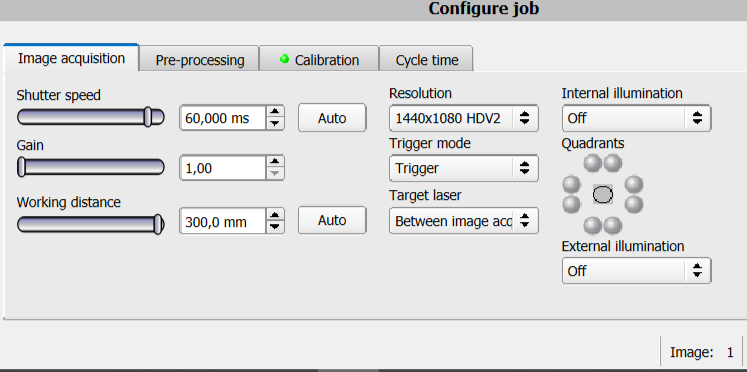
\includegraphics[width=\textwidth]{figures/job-configuration.png}
    \caption{Job configuration for the robotic camera}
    \label{fig:job-configuration-robotic}
\end{figure}

For a test specimen sheet metal type variant, a number of jobs are created during the camera configuration to fulfill the above mentioned tasks.
Figure \ref{fig:job-configuration-robotic} shows the job configuration for all the jobs in the robotic camera.
After calibration, a working distance of 300.0 mm is set. The is best operational distance for the camera from an object which has to be detected. The shutter speed varies from 15.0 ms, 30.0 ms, 45.0 ms, 60.0 ms, 75.0 ms and 90.0 ms. Thus, the camera takes a total of six captures with different shutter speed setting, if the default 60.0 ms shutter speed is unable to detect the sheet. A lower shutter speed value means less light will pass through the camera lens and the image will be darker in comparison to higher shutter speed settings. This setting is set in the cycle time tab.
Internal illumination is not used because of a large working distance. An external light is used to illuminate the sheet surface which is always on.


\begin{figure}[h]
    \centering
    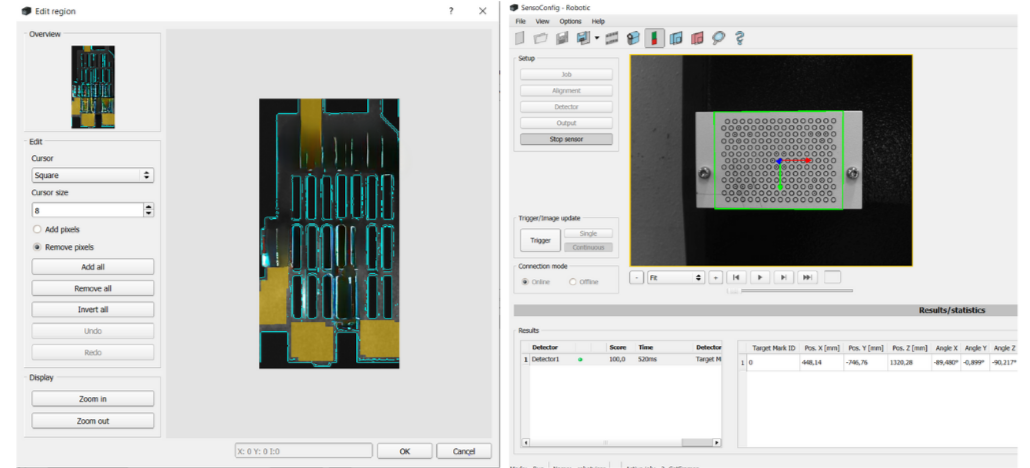
\includegraphics[width=\textwidth]{figures/robotic-detection.png}
    \caption{Using robotic camera for sheet detection (left) and marker detection (right)}
    \label{fig:robotic-detection}
\end{figure}

Mainly two detector methods are used by the robotic camera as shown in figure \ref{fig:robotic-detection}. These are detector contour and detector target mark 3D. \textbf{Detector Contour} locate and count objects by contours. An interesting region on the sheet metal part is marked for contouring. 
\textbf{Detector Target Mark 3D} locate objects in space using standarized markers (3D).
Whenever an object is detected by the camera, pose value of object is generated in world frame and sent over to the robot using telegram.